\mode<presentation>
{
  \usetheme{umbc4}
%  \setbeamercovered{dynamic}
}
\usepackage[english]{babel}
% or whatever

\usepackage[latin1]{inputenc}
% or whatever

\usepackage{times}
\usepackage[T1]{fontenc}
\usepackage{etex}
% Or whatever. Note that the encoding and the font should match. If T1
% does not look nice, try deleting the line with the fontenc.
%--------------------------------------------------------------------------------------------
%--- Other packages
\usepackage{pstricks}
\usepackage{pst-node}
\usepackage{pst-rel-points}
\usepackage{bcprules}
\usepackage{graphicx}
\newcommand{\change}[1]{{\red #1}}
%%%%%% Declarations Defined in custom-foils
%\setfootline{\insertshortauthor, \insertshortinstitute \hfill   \insertshorttitle \hfill \insertframenumber/\inserttotalframenumber} 
\newcommand{\mypart}[1]{%
  \frame[plain]{\mbox{}\vfill \psshadowbox{\huge #1} \vfill\mbox{}}
}
\author[karkare]{Amey Karkare \\ \url{karkare@cse.iitk.ac.in}}
\date[]{\scalebox{0.3}{\includegraphics{iitklogo.epsi}}}%
\institute[CSE, IITK]{\url{http://www.cse.iitk.ac.in/~karkare/cs738}\\Department of CSE, IIT Kanpur}
\title[CS738]{CS738: Advanced Compiler Optimizations}
\subtitle[]{}


\subtitle[Types]{\ \\{\LARGE Types and Program Analysis}}

\begin{document}

\frame{\titlepage}

\frame{
  \frametitle{Reference Book}
  Types and Programming Languages by Benjamin C. Pierce
}

\frame{
  \frametitle{Type: Definition}
  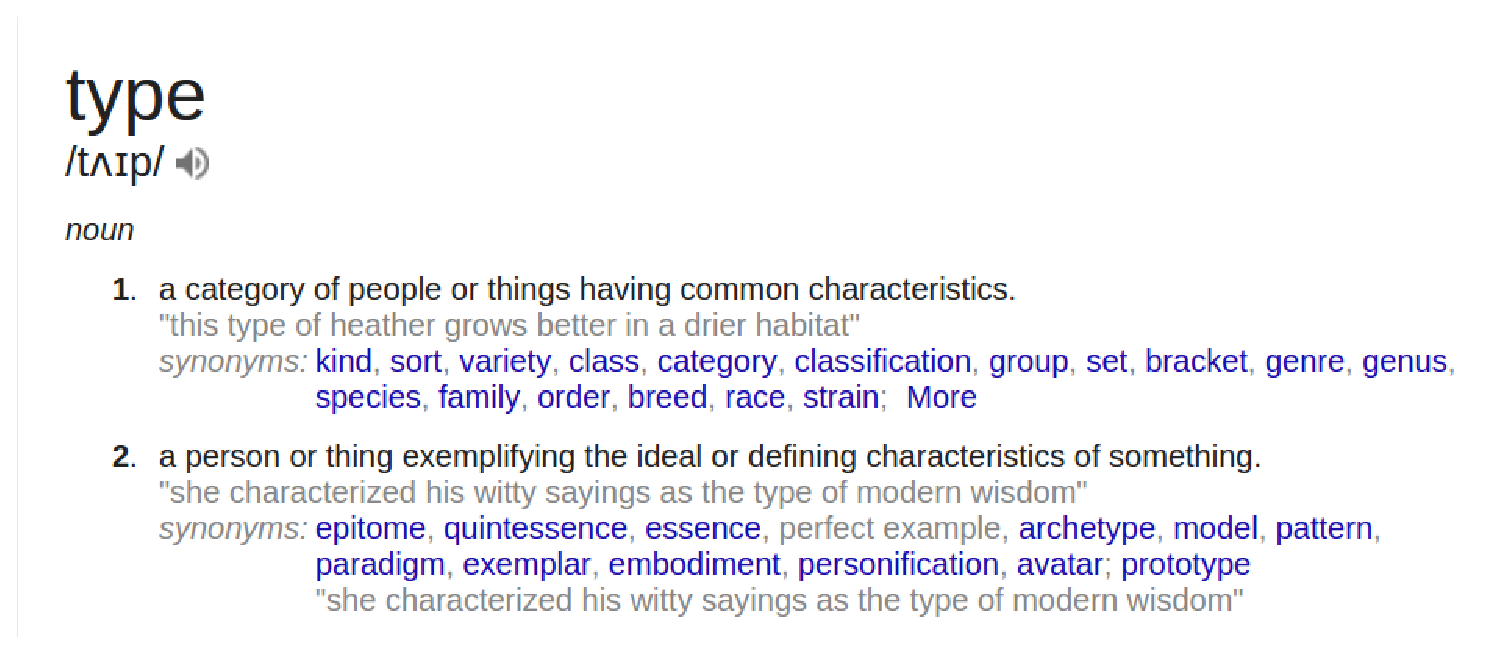
\includegraphics[width=\textwidth]{DefnOfTypes}
}

\frame{
  \frametitle{Types in Programming}
  \begin{itemize}[<+->]
  \item A collection of {\em values}
    \begin{center}
      $\scalebox{4}{+}$
    \end{center}
  \item The operations that are permitted on these values
  \end{itemize}
}

\frame{
  \frametitle{Type System}
  \begin{itemize}[<+->]
  \item A collection of rules for checking the correctness of usages of types
    \begin{itemize}
    \item ``Consistency'' of programs
    \end{itemize}
  \end{itemize}
}

\frame{
  \frametitle{The World of Programming Languages}
  \begin{itemize}[<+->]
  \item Typed
    \begin{itemize}
    \item C, C++, Java, Python, \ldots
    \end{itemize}
  \item Untyped
    \begin{itemize}
    \item Assembly, {\em any other?}
    \end{itemize}
  \end{itemize}
}

\frame{
  \frametitle{The World of Programming Languages}
  \begin{center}
    \begin{tabular}{l|p{3.5cm}|p{3.5cm}}\hline
      & {\bf Statically Typed} & {\bf Dynamically Typed} \\ \hline
      {\bf Strongly Typed} & \only<2->{ML, Haskell, Pascal (almost), Java (almost)} & \only<3->{Lisp, Scheme} \\ \hline
      {\bf Weekly Typed} & \only<4->{C, C++} & \only<5->{Perl} \\ \hline
    \end{tabular}
  \end{center}
}

\frame{
  \frametitle{Applications of Type-based Analyses}
  \begin{itemize}[<+->]
  \item Error Detection
    \begin{itemize}
    \item Language Safety
    \item Verification
    \end{itemize}
  \item Abstraction
  \item Documentation
  \item Maintenance
  \item Efficiency
  \end{itemize}
}

\newcommand{\tm}{{\bf \rm \Large t}}
\newcommand{\uif}{\mbox{\tt if}}
\newcommand{\uthen}{\mbox{\tt then}}
\newcommand{\uelse}{\mbox{\tt else}}
\newcommand{\usucc}{\mbox{\tt succ}}
\newcommand{\upred}{\mbox{\tt pred}}
\newcommand{\uiszero}{\mbox{\tt iszero}}
\newcommand{\utrue}{\mbox{\tt true}}
\newcommand{\ufalse}{\mbox{\tt false}}
\frame{
  \frametitle{Untyped Arithmetic Expression Language}
  \begin{tabular}{lp{.4\textwidth}l}
    \tm\ :=&& {\em -- terms} \\
    \pause & \utrue & {\em -- constant true} \\
    \pause & \ufalse & {\em -- constant false} \\
    \pause & \uif\ \tm\ \uthen\ \tm\ \uelse\ \tm & {\em -- conditional} \\
    \pause & 0 &  {\em -- constant zero} \\
    \pause & \usucc\ \tm & {\em -- successor} \\
    \pause & \upred\ \tm & {\em -- predecessor} \\
    \pause & \uiszero\ \tm & {\em -- zero test}
  \end{tabular}
}

\newcommand{\terms}{\ensuremath{\mathcal{T}}}
\frame{
  \frametitle{Syntax: Inductive Definition}
  The set of {\em terms} is the smallest set \terms\ such that
  \pause
  \begin{enumerate}[<+->]
  \item $\{\utrue, \ufalse, 0\} \subseteq \terms$
  \item if $\tm_1 \in \terms$, then 
    $\{\usucc\ \tm_1, \upred\ \tm_1, \uiszero\ \tm_1\} \subseteq \terms$
  \item   if $\tm_1 \in \terms$, $\tm_2 \in \terms$, and $\tm_3 \in \terms$ then
    $\uif\ \tm_1\ \uthen\ \tm_2\ \uelse\ \tm_3 \in \terms$    
  \end{enumerate}
}

\frame{
  \frametitle{Syntax: Inference Rules}
  The set of {\em terms}, \terms\, is defined by the following rules:\\[10pt]
  \pause
  \begin{minipage}{0.3\linewidth}
  \infax{\utrue \in \terms}    
  \end{minipage}
  \begin{minipage}{0.3\linewidth}
  \infax{\ufalse \in \terms}
  \end{minipage}
  \begin{minipage}{0.3\linewidth}
  \infax{0 \in \terms}
  \end{minipage}\\[10pt]
  \pause
  \begin{minipage}{0.3\linewidth}
  \infrule{\tm_1 \in \terms}{\usucc\ \tm_1 \in \terms}
  \end{minipage}
  \begin{minipage}{0.3\linewidth}
  \infrule{\tm_1 \in \terms}{\upred\ \tm_1 \in \terms}
  \end{minipage}
  \begin{minipage}{0.3\linewidth}
  \infrule{\tm_1 \in \terms}{\uiszero\ \tm_1 \in \terms}
  \end{minipage}\\[10pt]
  \pause
  \infrule{\tm_1 \in \terms \andalso \tm_2 \in \terms \andalso \tm_3 \in \terms}
  {\uif\ \tm_1\ \uthen\ \tm_2\ \uelse\ \tm_3 \in \terms}
}

\newcommand{\sterm}{\ensuremath{\mathcal{S}}}
\frame{
  \frametitle{Concrete Syntax}
  \begin{eqnarray*}
    \sterm_0 &=& \emptyset \\ \pause
    \sterm_{i+1} &=& \quad \{\utrue, \ufalse, 0\} \\ \pause
    & & \cup\ \{\usucc\ \tm_1, \upred\ \tm_1, \uiszero\ \tm_1 \mid \tm_1 \in \sterm_i\} \\ \pause
    & & \cup\ \{\uif\ \tm_1\ \uthen\ \tm_2\ \uelse\ \tm_3 \mid \tm_1, \tm_2, \tm_2 \in \sterm_i\}
  \end{eqnarray*} \pause
  Let $\sterm = \bigcup_i \sterm_i$. \\\pause
  Then, $\terms = \sterm$.
}

\newcommand{\consts}{\mbox{\em Consts}}
\newcommand{\size}{\mbox{\em size}}
\newcommand{\depth}{\mbox{\em depth}}

\frame{
  \frametitle{Induction on Terms}
  \begin{itemize}[<+->]
  \item Any $\tm \in \terms$
    \begin{itemize}
    \item Either a ground term, i.e. $\in \{\utrue, \ufalse, 0\}$
    \item Or is created from some smaller terms $\in \terms$
    \end{itemize}
  \item Allows for inductive definitions and inductive proofs.
  \item Three sample inductive properties
    \begin{itemize}
    \item \consts(t)
    \item \size(t)
    \item \depth(t)
    \end{itemize}
  \end{itemize}
}

\frame{
  \frametitle{\consts}
  \begin{itemize}
  \item The set of constants in a term \tm.
  \end{itemize}\pause
  \begin{eqnarray*}
    \consts(\utrue) &=& \{\utrue\} \\ \pause
    \consts(\ufalse) &=& \{\ufalse\} \\ \pause
    \consts(0) &=& \{0\} \\ \pause
    \consts(\usucc\ \tm) &=& \consts(\tm) \\ \pause
    \consts(\upred\ \tm) &=&  \consts(\tm)\\ \pause
    \consts(\uiszero\ \tm) &=&  \consts(\tm)\\ \pause
    \consts(\uif\ \tm_1\ \uthen\ \tm_2\ \uelse\ \tm_3) &=&  \consts(\tm_1) \\
    & & \cup\ \consts(\tm_2) \\ & & \cup\ \consts(\tm_3)
  \end{eqnarray*}
}

\frame{
  \frametitle{\size}
  \begin{itemize}
  \item The number of nodes in the abstract syntax tree of a term \tm.
  \end{itemize}\pause
  \begin{eqnarray*}
    \size(\utrue) &=& 1 \\ \pause
    \size(\ufalse) &=& 1 \\ \pause
    \size(0) &=& 1 \\ \pause
    \size(\usucc\ \tm) &=& \size(\tm) + 1 \\ \pause
    \size(\upred\ \tm) &=& \size(\tm) + 1\\ \pause
    \size(\uiszero\ \tm) &=&  \size(\tm) + 1\\ \pause
    \size(\uif\ \tm_1\ \uthen\ \tm_2\ \uelse\ \tm_3) &=&  \size(\tm_1) + \size(\tm_2)  + \size(\tm_3)
  \end{eqnarray*}
}

\frame{
  \frametitle{\depth}
  \begin{itemize}
  \item The maximum depth of the abstract syntax tree of a term \tm.
  \item Equivalently, the smallest $i$ such that $\tm \in \sterm_i$.
  \end{itemize}\pause
  \begin{eqnarray*}
    \depth(\utrue) &=& 1 \\ \pause
    \depth(\ufalse) &=& 1\\ \pause
    \depth(0) &=& 1 \\ \pause
    \depth(\usucc\ \tm) &=& \depth(\tm) + 1 \\ \pause
    \depth(\upred\ \tm) &=& \depth(\tm) + 1 \\ \pause
    \depth(\uiszero\ \tm) &=&  \depth(\tm) + 1 \\ \pause
    \depth(\uif\ \tm_1\ \uthen\ \tm_2\ \uelse\ \tm_3) &=&  \mbox{\rm max}(\depth(\tm_1) + \depth(\tm_2) \\ & & \qquad +\ \depth(\tm_3)) + 1
  \end{eqnarray*}
}

\frame{
  \frametitle{A Simple Property of Terms}
  \begin{itemize}[<+->]
  \item The number of distinct constants in a term \tm\ is no greater than the size of \tm.\[\left| \consts(\tm) \right| \leq \size(\tm)\]
  \item {\bf Proof:} Exercise.
  \end{itemize}
}

\newcommand{\val}{{\bf \rm \Large v}}
\frame{
  \frametitle{The Set of Values}
  \begin{tabular}{lp{.4\textwidth}l}
    \val\ :=&& {\em -- values} \\
    \pause & \utrue & {\em -- value true} \\
    \pause & \ufalse & {\em -- value false} \\
    \pause & 0 &  {\em -- value zero} \\
    \pause & \usucc\ \val & {\em -- successor value}
  \end{tabular}
}

\frame{
  \frametitle{Small-step Operational Semantics}
  \begin{itemize}
  \item $\tm \rightarrow \tm'$ denotes ``$\tm$ evaluates to $\tm'$ in one step''
  \end{itemize}\pause
  \infax{\uif\ \utrue\ \uthen\ \tm_2\ \uelse\ \tm_3 \rightarrow \tm_2}\pause
  \infax{\uif\ \ufalse\ \uthen\ \tm_2\ \uelse\ \tm_3 \rightarrow \tm_3}\pause
  \infrule{\tm_1 \rightarrow \tm_1'}{\uif\ \tm_1\ \uthen\ \tm_2\ \uelse\ \tm_3 \rightarrow \uif\ \tm_1'\ \uthen\ \tm_2\ \uelse\ \tm_3}
}

\frame{
  \frametitle{Small-step Operational Semantics (contd\ldots)}
  \begin{itemize}
  \item $\tm \rightarrow \tm'$ denotes ``$\tm$ evaluates to $\tm'$ in one step''
  \end{itemize}
  \infrule{\tm_1 \rightarrow \tm_1'}{\usucc\ \tm_1\ \rightarrow \usucc\ \tm_1'}\pause
  \infax{\upred\ 0 \rightarrow 0}\pause
  \infax{\upred\ (\usucc\ \val) \rightarrow \val}\pause
  \infrule{\tm_1 \rightarrow \tm_1'}{\upred\ \tm_1\ \rightarrow \upred\ \tm_1'}
}

\frame{
  \frametitle{Small-step Operational Semantics (contd\ldots)}
  \begin{itemize}
  \item $\tm \rightarrow \tm'$ denotes ``$\tm$ evaluates to $\tm'$ in one step''
  \end{itemize}
  \infax{\uiszero\ 0 \rightarrow \utrue}\pause
  \infax{\uiszero\ (\usucc\ \val) \rightarrow \ufalse}\pause
  \infrule{\tm_1 \rightarrow \tm_1'}{\uiszero\ \tm_1\ \rightarrow \uiszero\ \tm_1'}
}

\frame{
  \frametitle{Normal Form}
  \begin{itemize}[<+->]
  \item A term is $\tm$ in normal form if no evaluation rule applies to it.
  \item In other words, there is no $\tm'$ such that $\tm \rightarrow \tm'$.
  \end{itemize}
}

\frame{
  \frametitle{Evaluation Sequence}
  \begin{itemize}[<+->]
  \item An evaluation sequence starting from a term $\tm$ is a (finite or
    infinite) sequence of terms $\tm_1, \tm_2, \ldots$, such that\\
    \[\tm \rightarrow \tm_1\]
    \[\tm_1 \rightarrow \tm_2\]
    etc.
  \end{itemize}
}

\frame{
  \frametitle{Stuck Term}
  \begin{itemize}[<+->]
  \item A term is said to be {\bf stuck} if it is a normal form but not a value.
  \item A simple notion of ``run-time type error''
  \end{itemize}
}
\end{document}

